\section{Lösungen Herleiten}
\subsection{Umverteilung des Gewichtes}
Da der Lidar Sensor eine Neigung um \(7^\circ\) nach vorne hat (schwerer, ungestützter Vorbau), muss das Gewicht neu verteilt werden. Hierfür werden drei Möglichkeiten herausgearbeitet und in Tabelle~\ref{tab:nutzwert_gewicht} verglichen.

\subsubsection{Hochkante Einlage in den Mittelteil}
\paragraph{Art der Änderung}
\begin{itemize}
  \item Der Vorderbau wird mechanisch begradigt: die Bereiche um die Schraubpunkte werden abgefeilt, bis eine rechteckige, sauber einpassbare Form entsteht.
  \item Der Vorderbau wird anschließend hochkant in den Mittelteil integriert.
  \item Fixierung über einen Winkel hinter der Servolenkung, damit die Einheit verwindungssteif sitzt und Kräfte definiert eingeleitet werden.
  \item Das Batteriefach wird hochkant ausgerichtet und in Richtung Motor verschoben, um den Bauraum besser zu nutzen und den Schwerpunkt sinnvoll zu verlagern.
  \item Leitungsführung und Befestigungspunkte müssten dabei neu geplant werden, weil sich Einbauwinkel und Zugänglichkeit ändern.
\end{itemize}

\paragraph{Vorteile}
\begin{itemize}
  \item Sehr platzsparende Integration, kaum toter Bauraum.
  \item Wendekreis bleibt im Normalfall unverändert, da Radstand und Lenkeinschlag nicht zwangsläufig angepasst werden müssen.
  \item Konstruktion wirkt insgesamt kompakter und aufgeräumter, was spätere Erweiterungen erleichtern kann.
\end{itemize}

\paragraph{Nachteile}
\begin{itemize}
  \item Wartbarkeit kann schlechter werden: Akkuwechsel, Schrauben nachziehen, Komponenten tauschen wird je nach Einbauposition fummeliger.
  \item Höherer mechanischer Anpassungsaufwand (Feilen, Ausrichten, Winkel fertigen), dadurch mehr Risiko für Passungenauigkeiten.
  \item Kabelmanagement wird kritischer, weil weniger Platz für saubere Radien und Zugentlastung bleibt.
\end{itemize}

\subsubsection{Frankenstein Umbau}
\paragraph{Art der Änderung}
\begin{itemize}
  \item Vorderbau wird vollständig abgeschraubt.
  \item Mittelteil des Chassis wird durchgesägt, um eine neue Montageposition zu schaffen.
  \item Der Vorderbau wird in die Mitte versetzt und dort wieder verschraubt.
  \item Je nach Schnittstelle müssten Verstärkungen ergänzt werden (Platten, Winkel, zusätzliche Verschraubungen), damit die Struktur unter Last nicht nachgibt.
\end{itemize}

\paragraph{Vorteile}
\begin{itemize}
  \item Konzeptuell einfach, weil umsetzen und festschrauben als Grundidee klar ist.
  \item Kann schnell einen deutlichen Effekt auf Schwerpunkt und Platzverteilung bringen, ohne viele Detailarbeiten an einzelnen Bauteilen.
\end{itemize}

\paragraph{Nachteile}
\begin{itemize}
  \item Wendekreis kann schlechter werden, weil sich Geometrie und Gewichtsverteilung ungünstig verändern können.
  \item Stabilitätsrisiko: Durchsägen schwächt das Chassis, dadurch Verwindung, Risse, lockere Verschraubungen möglich.
  \item Oft mehr Nacharbeit als gedacht, weil nach dem groben Umbau Verstärkungen und Ausrichtung notwendig werden.
\end{itemize}

\subsubsection{Einkaufsrad Lösung}
\paragraph{Art der Änderung}
\begin{itemize}
  \item Ein Stützrad (Einkaufsrad) wird unter dem Vorderbau montiert.
  \item Ziel ist, dass das Rad einen Teil der Frontlast trägt und das Fahrzeug vorne mechanisch stabilisiert.
  \item Befestigung über eine einfache Halterung oder Montageplatte, ohne größere Eingriffe in den Aufbau.
\end{itemize}

\paragraph{Vorteile}
\begin{itemize}
  \item Sehr schnell und kostengünstig umsetzbar.
  \item Minimal invasiv: bestehender Aufbau bleibt weitgehend erhalten, Rückbau ist einfach.
  \item Sofortiger Effekt auf Lastverteilung, ohne Chassis oder Hauptbaugruppen umzubauen.
\end{itemize}

\paragraph{Nachteile}
\begin{itemize}
  \item Optisch eher Bastellösung, wirkt weniger integriert.
  \item Fahrverhalten kann schlechter werden: Nachlaufen, Flattern, zusätzliche Reibung, eingeschränkte Bodenfreiheit.
  \item Auf unebenem Untergrund oder bei Kanten kann das Stützrad stören oder hängen bleiben.
\end{itemize}

\subsubsection{Nutzwertanalyse zur Gewichtsumverteilung}
\begin{table}[htbp]
\centering
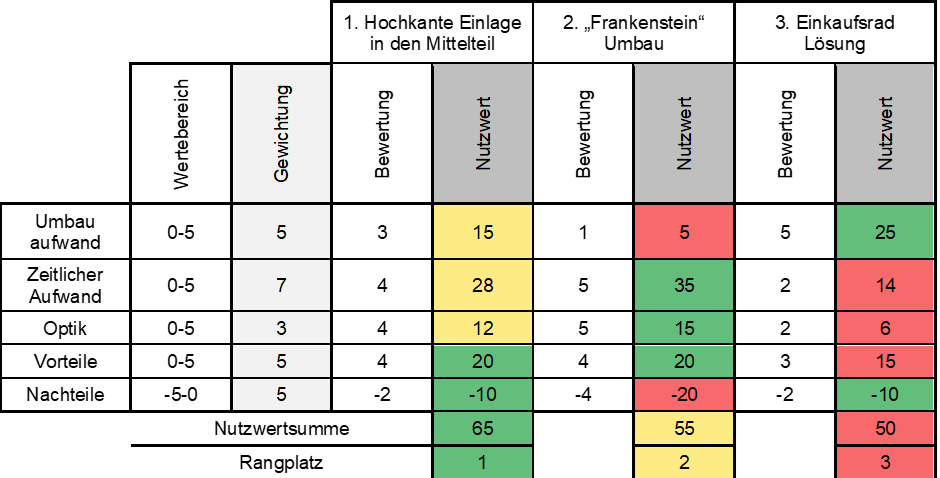
\includegraphics[width=\textwidth]{tables/Nutzweranalyse_Gewichtsverteilung.png}
\caption{Nutzwertanalyse zur Gewichtsverteilung}
\label{tab:nutzwert_gewicht}
\end{table}

Aus der Nutzwertanalyse in Tabelle~\ref{tab:nutzwert_gewicht} ergibt sich, dass die Hochkante Einlage im Mittelteil die beste Lösung zur Umverteilung des Gewichtes darstellt. Die Lösung bietet eine gute Balance aus Umsetzbarkeit, Fahrverhalten und Wartbarkeit, während sie gleichzeitig den Schwerpunkt effektiv verlagert. Obwohl der mechanische Anpassungsaufwand höher ist, überwiegen die Vorteile in Bezug auf Platznutzung und Fahrzeugperformance. Daher wird diese Lösung für die weitere Umsetzung empfohlen. 

\newpage
\subsection{Gegenständen ausweichen}
\subsubsection{Mathematische Formeln für die Berechnung der Fahrbahn}
Bei der mathematischen Modellierung von Trajektorien zur Umfahrung eines Hindernisses spielt die Wahl der zugrunde liegenden Funktion eine entscheidende Rolle.
Insbesondere sind Aspekte wie Krümmungsverhalten, lokale Anpassungsfähigkeit und das asymptotische Verhalten von großer Bedeutung.
Im Folgenden werden Parabeln, Exponentialfunktionen und die Gaußsche Glockenkurve im Hinblick auf ihre Eignung zur Umfahrung eines Gegenstandes verglichen.

\subsubsection*{Parabeln}
Eine Parabel ist eine ganzrationale Funktion zweiten Grades der Form
\[
f(x) = ax^2 + bx + c.
\]
Sie besitzt genau einen Scheitelpunkt und eine konstante zweite Ableitung. Diese konstante Krümmung führt dazu, dass das auto nicht gerade auf einen Gegenstand zu fahren kann, ihn umfahren und wieder zurück auf seine ausgangsspur zurück fahren kann nach dem Umfahren. Eine Parabel wäre daher nur bedingt geeignet um vor einem Gegenstand umzudrehen falls der Gegenstand nicht umfahrbar ist.
\\
\begin{figure}[htbp]
\centering
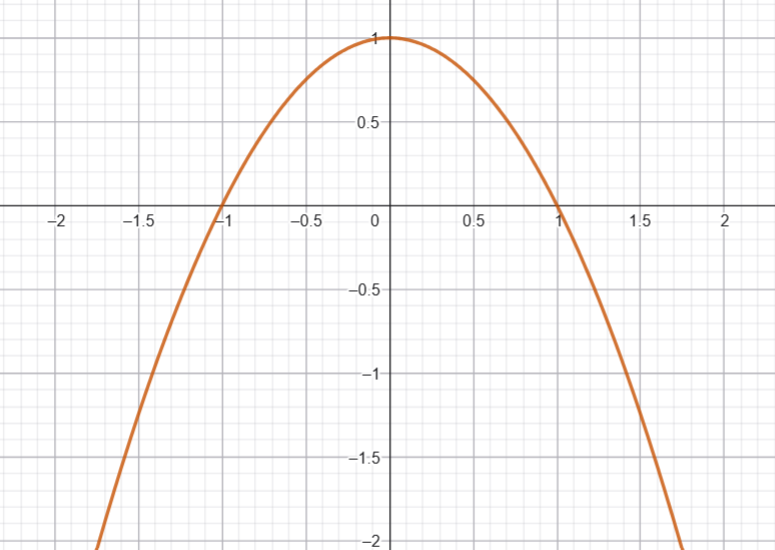
\includegraphics[width=0.5\textwidth]{Images/Parabel.png}
\caption{Parabel Funktion}
\label{fig:parabel}
\end{figure}
\\

\subsubsection*{Exponentialfunktionen}
Exponentialfunktionen der Form
\[
f(x) = a \cdot e^{bx}
\]
zeigen ein stark asymmetrisches Verhalten. Sie besitzen keinen Scheitelpunkt und keine natürliche Symmetrieachse. Das Wachstum bzw. der Abfall erfolgt einseitig sehr stark, während auf der anderen Seite nur eine geringe Änderung stattfindet.
Für die Umfahrung eines Gegenstandes ist diese Eigenschaft nachteilig, da eine ausgewogene seitliche Auslenkung benötigt wird. Exponentialfunktionen erzeugen entweder eine zu abrupte oder eine zu flache Richtungsänderung und erlauben keine kontrollierte Rückführung auf die ursprüngliche Spur. Allerdings könnten sie in speziellen Fällen, z.B. bei sehr engen Hindernissen, als Notfallmanöver eingesetzt werden, um schnell Kurven zu fahren, wenn keine andere Option besteht.
\begin{figure}[htbp]
\centering
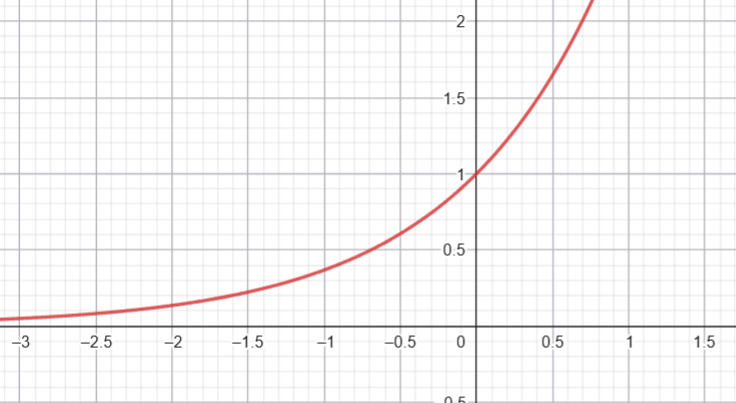
\includegraphics[width=0.5\textwidth]{Images/Expondential Funktion.png}
\caption{Expondential Funktion}
\label{fig:expondential_funktion}
\end{figure}
\newpage

\subsubsection*{Gaußsche Glockenkurve}
Die Gaußsche Glockenkurve ist definiert durch
\[
f(x) = A \cdot e^{-\frac{(x-\mu)^2}{2\sigma^2}}.
\]
Sie besitzt einen klar definierten Scheitelpunkt bei $x = \mu$, ist streng symmetrisch und fällt beidseitig sanft gegen null ab. Diese Eigenschaften machen sie besonders geeignet für die Umfahrung von Hindernissen.
Die Ausweichbewegung ist lokal begrenzt, kontinuierlich differenzierbar und verursacht keine abrupten Richtungsänderungen. Gleichzeitig wird der ursprüngliche Fahrweg nach dem Umfahren des Hindernisses automatisch wieder angenähert.
\begin{figure}[htbp]
\centering
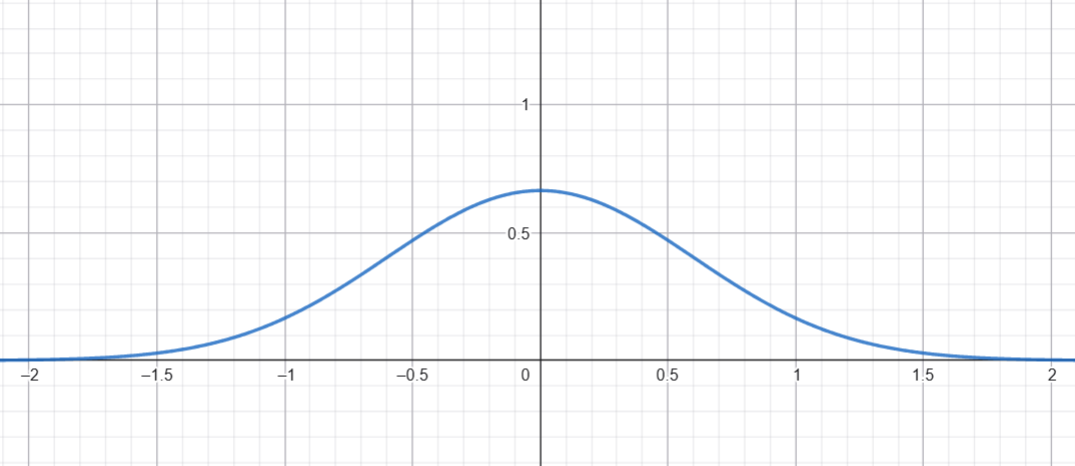
\includegraphics[width=0.5\textwidth]{Images/Gaussche Glocke.png}
\caption{Gaussche Glocke Funktion}
\label{fig:gaussche_glocke}
\end{figure}
Ein weiterer entscheidender Vorteil der Gaußschen Glockenkurve ergibt sich durch ihre rekursive Anwendung. Wird nach der Umfahrung eines Hindernisses am Scheitelpunkt der resultierenden Kurve erneut eine Gaußfunktion angesetzt, so können auch komplexe Hindernisformen oder mehrere aufeinanderfolgende Objekte zuverlässig umfahren werden.
Durch diese rekursive Überlagerung entsteht eine adaptive Fahrtenkurve, die sich flexibel an nahezu jede Umgebung anpassen kann. Unter der Voraussetzung ausreichender Parameteranpassung ist es damit theoretisch möglich, um jeden Gegenstand herumzufahren.
\newpage

\subsubsection*{Fazit}
Zusammenfassend lässt sich sagen, dass die Gaußsche Glockenkurve aufgrund ihrer symmetrischen Form, der lokalen Begrenzung und der sanften Krümmung die beste Wahl für die Umfahrung von Gegenständen darstellt. Parabeln können in bestimmten Situationen nützlich sein, bieten jedoch nicht die notwendige Flexibilität und Kontrolle. Exponentialfunktionen sind für diesen Anwendungsfall weniger geeignet, da sie zu einseitig und abrupt reagieren. Die Möglichkeit der rekursiven Anwendung der Gaußschen Glockenkurve ermöglicht es zudem, komplexe Hindernisformationen effektiv zu bewältigen, was sie zur optimalen Lösung für die Fahrbahnplanung bei der Umfahrung von Gegenständen macht.
Damit ein optimales Fahrverhalten erreicht wird, sollten die Parameter der Gaußschen Glockenkurve sorgfältig angepasst werden, um eine harmonische und sichere Umfahrung zu gewährleisten. Dabei ist wichtig zu beachten, dass die  Wahl der kurvensteigung nicht über den maximalen Lenkeinschlag hinausgehen darf, um die Fahrstabilität zu gewährleisten. Insgesamt bietet die Gaußsche Glockenkurve eine robuste und flexible Grundlage für die Entwicklung von Algorithmen zur Hindernisumfahrung in autonomen Fahrsystemen.

\subsubsection{Berechnung Lenkwinkel}
Die Berechnung des Lenkwinkels für die Umfahrung eines Gegenstandes basiert auf der geometrischen Beziehung zwischen der Fahrbahnkurve und der Fahrzeugdynamik. Angenommen, die Fahrbahn wird durch eine Funktion \(f(x)\) beschrieben, die die seitliche Auslenkung in Abhängigkeit von der Vorwärtsbewegung \(x\) angibt, kann der Lenkwinkel \(\delta\) wie folgt berechnet werden:
\[\delta(x) = \arctan\left(\frac{df}{dx}\right).\]
Hierbei ist \(\frac{df}{dx}\) die erste Ableitung der Fahrbahnfunktion, die die Steigung der Kurve an einem bestimmten Punkt \(x\) angibt. Der Lenkwinkel \(\delta\) wird in Radiant oder Grad angegeben und gibt an, wie stark das Fahrzeug in diesem Moment lenken muss, um der Fahrbahn zu folgen.
Die Berechnung des Lenkwinkels ist entscheidend für die Steuerung des Fahrzeugs und die Gewährleistung einer sicheren Umfahrung des Gegenstandes. Es ist wichtig, dass der berechnete Lenkwinkel innerhalb der mechanischen Grenzen des Fahrzeugs liegt, um eine Übersteuerung oder Untersteuerung zu vermeiden. Zudem sollte die Berechnung in Echtzeit erfolgen, um auf dynamische Veränderungen in der Umgebung reagieren zu können. Die Implementierung dieser Berechnung erfordert eine genaue Modellierung der Fahrzeugdynamik und eine präzise Erfassung der Fahrbahnkurve, um eine effektive und sichere Umfahrung zu gewährleisten.
\end{document}